%%%%%%%%%%%%%%%%%%%%%%%%%%%%%%%%%%%%%%%%%%%%%%%%%%%%%%%%%%%%%%%%%%%%%%%%%%%%%%
%
%  surfactant.tex
%
%  Some notes on surfactant work
%
%%%%%%%%%%%%%%%%%%%%%%%%%%%%%%%%%%%%%%%%%%%%%%%%%%%%%%%%%%%%%%%%%%%%%%%%%%%%%%

\section{Surfactants}

This section describes the approach taken to study surfactants. Here,
we always adopt the hydrid method, i.e., LB for the hydrodynmic
equations and finite difference for the associated Cahn-Hilliard
equations. Coupling between the two sectors is via the velocity
field and the external force on the fluid computed via the
divergence of the `chemical stress'.

In this model the surfactant appears as a concentration field
$\psi(\mathbf{r};t)$, alongside the compositional order parameter
$\phi(\mathbf{r};t)$ as appears in the binary fluid. There are
two corresponding Cahn-Hilliard equations: first,

\begin{equation}
\partial_t \phi + \partial_\alpha \phi u_\alpha = 
\partial_\alpha M_\phi \partial_\alpha \mu_\phi,
\end{equation}
and second
\begin{equation}
\partial_t \psi + \partial_\alpha \psi u_\alpha = 
\partial_\alpha M_\psi \partial_\alpha \mu_\psi.
\end{equation}

\subsection{Free Energy}

A number of different free energies have been used to study
surfactants [cite Yeomans]. Here, the free energy is based on
that used by van der Graff and van der Sman and others [cite].
There are a number of different contributions to the free
energy density:
\begin{equation}
f = f_\phi + f_\psi +f_1 + f_{ex}.
\end{equation}
The first is exactly that used for the binary fluid, i.e.,
\begin{equation}
f_\phi (\phi, \partial_\alpha\phi) =
{\textstyle \frac{1}{2}} A \phi^2 + {\textstyle \frac{1}{4}} B \phi^4
+ {\textstyle \frac{1}{2}} \kappa (\partial_\alpha \phi)^2.
\end{equation}
The surface tension and the interfacial width are determined from the
choice of parameters $A,B,\kappa$ as before.
The second term in the free energy density
represents the entropic
energy of mixing of the surfactant with the bulk phases
\begin{equation}
f_\psi (\psi) = kT \left[ \psi \ln\psi + (1 - \psi)\ln(1-\psi) \right]
\end{equation}
where the parameter $kT$ sets the energy scale for the whole system.
The surfactant order parameter, $\psi$, is unity for a saturated
interface and zero for a plain interface.

The surfactant lowers the energy of the interface where it is adsorbed
there, represented by the term
\begin{equation}
f_1(\psi, \partial_\alpha \phi) 
= -{\textstyle \frac{1}{2}} \epsilon \psi (\partial_\alpha \phi)^2
  -{\textstyle \frac{1}{2}} \beta  \psi^2 (\partial_\alpha \phi)^2
\end{equation}
where $\epsilon$ and $\beta$ are parameters. Note that only the
first term appears in \cite{vandergraaf}, while the second term is
based on that appearing in, e.g., \cite{diamant}. If $\beta = 0$,
the surfactant profile at the interface is symmetric (so-called
Langmuir adsoption) whereas the term in $\beta$ induces an
asymmetry (Frumpkin adsorption).
Finally,  $f_{ex}$ is [van der Sman claims]
an enthalpic contribution introduced 
to stabilise the interface \cite{theissengompper}
\begin{equation}
f_{ex} (\psi, \partial_\alpha \phi) = {\textstyle\frac{1}{2}} W \psi \phi^2,
\end{equation}
with $W$ a parameter.

\subsection{Chemical potentials}

The respective chemical potentials are obtained from the functional
derivatives of the free energy $\mu_\phi = \delta F / \delta \phi$ and
$\mu_\psi = \delta F / \delta \psi$. We obtain:
\begin{equation}
\mu_\phi =
A\phi + B\phi^3 -\kappa \partial_\alpha^2 \phi
+ W\psi\phi + \epsilon\psi\partial_\alpha^2 \phi
+ \epsilon \partial_\alpha \phi \partial_\alpha \psi
+ 2\beta \psi\partial_\alpha\phi \partial_\alpha \psi
+ \beta \psi^2 \partial_\alpha^2 \phi,
\end{equation}
and
\begin{equation}
\mu_\psi = kT \left[ \ln\psi - \ln(1-\psi) \right]
+ {\textstyle \frac{1}{2}}W\phi^2
- {\textstyle \frac{1}{2}}\epsilon (\partial_\alpha \phi)^2
- \beta\psi (\partial_\alpha \phi)^2.
\end{equation}
As before, the pressure tensor is $P_{\alpha\beta} = p_0\delta_{\alpha\beta}
+ \tilde{P}_{\alpha\beta}$ with the isotropic part being determined as (e.g.,
\cite{theissengompper})
\begin{equation}
p_0 = \phi \mu_\phi + \psi \mu_\psi - f(\phi, \psi, \partial_\alpha \phi).
\end{equation}
There is no closed form for the tensor part, which must be chosen to
comply with the constraint that in mechanical equilibrium
\begin{equation}
\partial_\alpha P_{\alpha\beta} = (\phi\partial_\alpha\mu_\phi +
\psi\partial_\alpha\mu_\psi)\delta_{\alpha\beta}.
\end{equation}
In this way we obtain for the isotropic contribution
\begin{eqnarray}
p_0 = {\textstyle \frac{1}{2}}A\phi^2 + {\textstyle \frac{3}{4}}B\phi^4 
- {\textstyle\frac{1}{2}}\kappa (\partial_\alpha\phi)^2 
- \kappa \phi \partial_\alpha^2 \phi
- kT \ln(1-\psi) + W\psi\phi^2
\nonumber\\
+ \epsilon \phi \partial_\alpha \phi \partial_\alpha \psi
+ \epsilon\phi\psi \partial_\alpha^2 \phi
+ 2 \beta\phi\psi \partial_\alpha \phi \partial_\alpha\psi
+ \beta \phi \psi^2 \partial_\alpha^2 \phi
- {\textstyle\frac{1}{2}} \beta \psi^2 (\partial_\alpha \phi)^2
\end{eqnarray}
and for the tensor part we can have
\begin{equation}
\tilde{P}_{\alpha\beta} =
(\kappa - \epsilon \psi - \beta\psi^2) 
\partial_\alpha \phi \partial_\beta \phi.
\end{equation}

\subsection{Note on Experimental Measurements}

Experimental measurements have generally been based on mechanical
methods which allow the determination of an interfacial tension
(for recent reviews, see \cite{chang,eastoe}). The degree of surface
activity is then accessed by measuring the the interfacial tension
$\sigma$ as a function of the bulk concentration $\psi_b$, and then
using the Gibbs equation
\begin{equation}
\psi_{0,\mathrm{eq}} = -\frac{1}{nRT}
\left( \frac{\partial \sigma}{\partial \ln \psi_b} \right)_T
\end{equation}
where $\psi_{0,\mathrm{eq}}$ is the equilibrium surface excess
concentration. The curve of $\psi_{0,\mathrm{eq}}$ against $\psi_b$
so obtained is thus relevant for a fixed temperature and is generally
refered to as the \textit{adsorption isotherm}. More recently, the
method of neutron reflection has been used to to access the interfacial
concentration directly (with good agreement with the mechanical
methods).

\subsubsection{Dynamic surface tension}

A newly formed interface (e.g., after shaking) in a surfactant
solution will have interfacial tension close to the bare value
$\sigma_0$. As the surfactant concentration at the interface
approaches its equilibrium value, the interfacial tension is
reduced. The quantity of interest is then the \textit{dynamical
surface tension} $\sigma(t)$. This process takes place on
timescales typically 10$^{-3}$--1 second, and is important in
many industrial processes such as coatings and formation of
soap lather.

At equilibrium, the final change in interfacial tension can
be obtained from Gibbs' equation together with a suitable
isotherm relating $\psi_0$ and $\psi_b$. 

\subsubsection{Adsorption isotherms}

A simple choice of isotherm is Henry's law:
\begin{equation}
\psi_{0,\mathrm{eq}} = K_H \psi_b
\label{eq:iso:henry}
\end{equation}
where $K_H$ is the equilibrium adsorption constant. Note this has the
dimensions of length, and represents the thickness of bulk solution
holding the same quantity of surfactant as an interface with
concentration $\psi_{0,\mathrm{eq}}$. In this way it is also a
measure of the strength of surface activity for a given surfactant.
Henry's law has a number of drawbacks: there is no upper limit
on $\psi_0$, and is only valid at low concentrations.

A more practical choice is the Langmuir equilibrium isotherm
\begin{equation}
\psi_{0,\mathrm{eq}} = \psi^\star \frac{K_L \psi_b}{1 + K_L \psi_b}
\label{eq:iso:langmuir}
\end{equation}
where $\psi^\star$ is the maximum concentration supported at the
interface and the Langmuir equilibrium adsorption constant is $K_L$
(with units mol$^{-1}$~m$^3$). At low concentrations $ K_L\psi_b << 1$,
the Langmuir isotherm reduces to the Henry isotherm with
$K_H = \psi^\star K_L$.

One further case of interest here is the Frumkin isotherm
\begin{equation}
\psi_{0, \mathrm{eq}} = \psi^\star
\frac{K_F \psi_b}{K_F\psi_b + e^{-B\psi_{0,\mathrm{eq}} / \psi^\star}}
\label{eq:iso:frumkin}
\end{equation}
where the Frumkin equilibrium adsorption constant $K_F$ again
has units of mol$^{-1}$~m$^3$. The dimensionless parameter $B$
 is a measure of the degree to which the surfactant behaviour
at the interface is non-ideal. For $B=0$, the Frumkin isotherm
reduces to that of Langmuir.

\subsection{Note on the Theory of Diamant and Andelman 1996}

As we ultimately adopt a free energy approach, we first review one
free energy based work --- that of Diamant and Andelman
\cite{diamant96}. This introduces a uniform system with interface
of zero thickness at $z = 0$. A uniform dilute solution of
surfactant occupies $z > 0$. The excess free energy per unit area
of interface is then written
\begin{equation}
\Delta\sigma [\psi] = \int_0^\infty  \big\{ \Delta f[\psi (z)] +
f_0 [\psi (z) ] \delta(z)  \big\} \mathrm{d}z. 
\end{equation}
The first term here is a contribution from the bulk while the
second is that from the interface. 

The uniform bulk solution has an ideal entropy of mixing
\begin{equation}
\Delta f(\psi) = (1/a^3)
\big\{ kT[\psi \ln\psi - \psi - (\psi_b \ln\psi_b - \psi_b)]
- \mu_b (\psi - \psi_b) \big\}.
\label{eq:da2}
\end{equation}
Here, $a$ is the characteristic size of the surfactant molecules.
The chemical potential $\mu_b$ and volume fraction of surfactant
in the bulk are fixed (with $\psi_b < 1$). The final term in
Eq.~\ref{eq:da2} is a contact term with a reservoir at $z = \infty$.

At the interface, we have a surfactant concentration $\psi_0$, which
is no longer small:
\begin{equation}
f_0 (\psi_0) = (1/a^2) \big\{
kT [ \psi_0 \ln\psi_0 + (1 - \psi_0) \ln(1 - \psi_0)]
- \alpha\psi_0 - {\textstyle\frac{1}{2}}\beta\psi_0^2 - \mu_1\psi_0 \big\}.
\end{equation} 
The first term is the full entropy of mixing. The second term represents
the reduction ($\alpha$ is positive) in surface energy owing to the
presence of surfactant. The third term represents an attractive
interaction between surfactants at the interface ($beta$ again positive).
The final term is a contact term between the interface and the adjacent
solution (at $z\rightarrow 0$).

\subsubsection{Equilibrium}

At equilibrium, where the chemical potential is the same throughout
the system $\mu (z) = \mu_b$, the DA recover the adsorption isotherm
\begin{equation}
\psi_{0,\mathrm{eq}} = \frac{\psi_b}{\psi_b
+ e^{-(\alpha + \beta\psi_{0,\mathrm{eq}})/kT}}.
\label{eq:iso:diamant}
\end{equation}
Comparison with the experiment forms Eq.~\ref{eq:iso:langmuir} and
Eq.~\ref{eq:iso:frumkin} reveals that $K_F$ is equivalent to
$e^{\alpha /kT}$ in the Frumkin isotherm. In addition, the equilibrium
equation of state is
\begin{equation}
\Delta \gamma_{\mathrm{eq}} = (1/a^2) [ kT \ln (1 - \psi_0) 
+ {\textstyle\frac{1}{2}}\beta \psi_0^2 ].
\end{equation}

\subsubsection{Out of Equilibrium}

DA96 go on to derive a variant of the Ward-Tordai equation \cite{wardtordai}
which describes the time evolution of the concentration of surfactant
at the interface:
\begin{equation}
\psi_0 (t) = \sqrt{D/\pi a^2}
\Bigg[ 2\psi_b \sqrt{t} 
- \int_0^\infty \frac{\psi_1 (\tau)}{\sqrt{t - \tau}} \mathrm{d}\tau \Bigg]
+ 2\psi_b - \psi_1.
\label{eq:wardtordai}
\end{equation}
When the time-scale for equilibration at the interface is fast compared
with that in the bulk, $\psi_0$ responds immediately to changes in
$\psi_1$. This is the case of \textit{diffusion limited adsorption} (DLA).
Here, the diffusive problem Eq.~\ref{eq:wardtordai} can be closed
using the isotherm Eq.~\ref{eq:iso:diamant} with $\psi_b$ replaced by
$\psi_1$. This can be solved numerically for $\psi_0 (t)$. If one further
makes the assumption that the equilibrium equation of state holds
approximately out of equililbrium, then one can also recover
$\Delta\gamma (t)$, that is, the dynamic surface tension.

\subsection{Current Model}

The current model is based the standard symmetric binary fluid
free energy to represent two fluids separated by a finite
interface of thickness $\xi_0$. This free energy is the usual
functional of the compositional order parameter $\phi$. This is
referred to as
\begin{equation}
f_\phi = {\textstyle\frac{1}{2}}A\phi^2
+ {\textstyle\frac{1}{4}}B\phi^4
+ {\textstyle\frac{1}{2}}\kappa (\partial_\alpha \phi)^2.
\end{equation}
Note that here, the excess free energy related to $f_\phi$ may
be integrated analytically to provide an expression for the
intefacial tension $\sigma_0 = 4\kappa\phi^\star/3\xi_0$ at
equilibrium.
(In one dimension the equiibrium profile
is $\phi(z) = \phi^\star \tanh(z/\xi_0)$ with $\phi^\star = \sqrt{-A/B}$
and $\xi_0^2 = -2\kappa/A$.)

To this we add a separate order parameter to represent the
surfactant $\psi$ \cite{vandergraaf}. The free energy density
is made up of two parts following DA96:
\begin{equation}
f_{\psi} = kT[\psi\ln\psi  + (1 - \psi) \ln (1 - \psi)]
\end{equation}
represents the entropy of mixing, valid in both the bulk and at
the interface. The interfacial part of the free energy density is
\begin{equation}
f_{\psi,i} = -{\textstyle\frac{1}{2}}\epsilon\psi (\partial_\alpha \phi)^2
- {\textstyle\frac{1}{2}} \beta \psi^2 (\partial_\alpha \phi)^2.
\end{equation}

We note that the excess free energy can no longer be integrated
exactly. However, it can be integrated numerically for a
given profile $\psi(z)$ (see below).

\subsubsection{Equilibrium}

We can compute the chemical potential associated with each order
parameter by taking the functional derivative with respect to
$\phi$ and $\psi$ respectively:
\begin{equation}
\mu_\phi = A\phi + B\phi^3 - \kappa \partial_\alpha^2 \phi
+ \epsilon \partial_\alpha \phi \partial_\alpha \psi
+ \epsilon \psi \partial_\alpha^2 \phi
+ 2\beta\psi \partial_\alpha \phi \partial_\alpha \psi
+ \beta\psi^2 \partial_\alpha^2 \phi,
\label{eq:mu:phi}
\end{equation}
and
\begin{equation}
\mu_\psi = kT[\ln\psi - \ln(1 - \psi)]
- {\textstyle \frac{1}{2}} \epsilon (\partial_\alpha \phi)^2
- \beta\psi (\partial_\alpha \phi)^2.
\label{eq:mu:psi}
\end{equation}

At equilibrium, we can set the chemical potential in the bulk and
at the interface to be equal. We assume that the presence of
surfactant does not affect the form of the equilibrium
composition profile so that in one dimension
$\phi(z) = \phi^\star \tanh(z/\xi_0)$ as before.
In the bulk we assume the concentration $\psi_b << 1$ so that
Eq.~\ref{eq:mu:psi} gives $\mu_{\psi,b} = kT\ln \psi_b$. At
the interface we ahve $\mu_{\phi,i} = kT[\ln\psi_0 - \ln(1 - \psi_0)]
- (1/2)\epsilon(\partial_\alpha \phi)^2
- \beta\psi_0 (\partial_\alpha \phi)^2$.
If we equate $\mu_{\psi, b}$ and $\mu_{\psi,i}$ we can recover the
Frumkin isotherm
\begin{equation}
\psi_{0,\mathrm{eq}} = \frac{\psi_b}{\psi_b +
e^{-({\scriptscriptstyle \frac{1}{2}}\epsilon + \beta\psi_{0,\mathrm{eq}})
(\phi^\star)^2 / \xi_0^2 kT}}.
\end{equation}
This is equivalent to Eq.~\ref{eq:iso:diamant} of DA96, where the
interfacial width has has appeared in place of $a$ (absorped into
the definition of the free energy density by DA96).


In the following we have $D = M_\psi \psi ( 1 - \psi)$. The
initial interfacial width is $\xi = 1.13$ (narrower than the
equilibrium value). This is a one-dimensional system of
length 100 lattice units. We choose to fix the binary fluid
parameters, and fix $\epsilon$ in relation to $\kappa$. The
isotherm is then varied by adjusting the value of $kT$.

\subsubsection{Parameters with $\mathbf{\xi_0 = 1.13}$, $\epsilon = \kappa/4$}

Here we keep the standard binary fluid parameters, having interfacial
width $\xi_0 = 1.13$.

\begin{table}[h]
\begin{center}
\begin{tabular}{|c|c|c|c|c|c|c|c|c|c|}
\hline
Name & $\eta$ & $-A,B$ & $\kappa$ & $kT$ & $\epsilon$ & $\beta$ & $W$
     & $M$ & $M_\psi$\\
\hline
R008a & 1/6 & 0.0625 & 0.04 & 1.6965$\times 10^{-3}$ & 0.01 & 0.0000 & 0.0 
      & 0.15 & 1.0 \\
R008d &  &  &  & & & 0.0025 &  &  &  \\
\hline
R006a & 1/6 & 0.0625 & 0.04 & 8.48231$\times 10^{-4}$ & 0.01 & 0.0000 & 0.0 
      & 0.15 & 1.0 \\
R006d & &  &  &  & & 0.0025 &  &  &  \\
\hline
R010a & 0.025 & 0.00625 & 0.004 & 1.6965$\times 10^{-4}$ & 0.001
      & 0.0000 & 0.0 & 2.0 & 2.0 \\
R010d & &  &  &  & & 0.0005 &  &  &  \\
\hline
R012a & 0.025 & 0.00625 & 0.004 & 8.48231$\times 10^{-5}$ & 0.001
      & 0.0000 & 0.0 & 2.0 & 2.0 \\
R012d & &  &  &  & & 0.0005 &  &  &  \\
\hline
\end{tabular}
\caption{Parameters for $\xi_0 = 1.13$ and $\epsilon = \kappa/4$.}
\end{center}
\end{table}



\subsubsection{Parameters with $\mathbf{\xi_0 = 2.26}$, $\epsilon = \kappa/4$}

Here we relax the interfaical width by a factor of 2, but
keep $A,-B$ as before so that the surface tension is increased
by a factor of $\sqrt{2}$.

\begin{table}[h]
\begin{center}
\begin{tabular}{|c|c|c|c|c|c|c|c|c|c|}
\hline
Name & $\eta$ & $-A,B$ & $\kappa$ & $kT$ & $\epsilon$ & $\beta$ & $W$
     & $M$ & $M_\psi$\\
\hline
R002a & 1/6 & 0.0625 & 0.16 & 1.6965$\times 10^{-3}$ & 0.04 & 0.00 & 0.0 
      & 0.15 & 1.0 \\
R002d &  &  &  & & & 0.01 &  &  &  \\
R002f &  &  &  & & & 0.02 &  &  &  \\
\hline
R003a & 1/6 & 0.0625 & 0.16 & 5.6549$\times 10^{-4}$ & 0.04 & 0.00 & 0.0 
      & 0.15 & 1.0 \\

R003d & &  & &  &  & 0.01 &  &  & 1.0\\
R003e & &  & &  &  & 0.01 &  &  & 0.5\\
R003f & &  & &  &  & 0.02 &  &  & 1.0\\
\hline
R004a & 1/6 & 0.0625 & 0.16 & 8.48231$\times 10^{-4}$ & 0.04 & 0.00 & 0.0 
      & 0.15 & 1.0 \\
R004d & &  &  &  & & 0.01 &  &  &  \\
R004f & &  &  &  & & 0.02 &  &  &  \\

\hline
\end{tabular}
\caption{Parameters for the surfactant free energy model. There are
three values of the (Langmuir) isotherm $(1/K_L) = 0.1$ (R002a),
0.01 (R004a) and 0.001 (R003a).
See section X for notes on $W$.}
\end{center}
\end{table}


In the following we retain $\xi_0 = 2.26$ but keep the same surface
tension cf. $\xi_0 = 1.13$, that is 0.047.

\begin{table}[h]
\begin{center}
\begin{tabular}{|c|c|c|c|c|c|c|c|c|c|}
\hline
Name & $\eta$ & $-A,B$ & $\kappa$ & $kT$ & $\epsilon$ & $\beta$ & $W$
     & $M$ & $M_\psi$\\
\hline
R022a & 1/6 & 0.03125 & 0.08 & 8.48231$\times 10^{-4}$ & 0.02 & 0.000 & 0.0 
      & 0.15 & 2.0 \\
R022d &  &  &  & & & 0.005 &  &  &  \\
\hline
R024a & 1/6 & 0.03125 & 0.08 & 4.24115$\times 10^{-4}$ & 0.02 & 0.00 & 0.0 
      & 0.15 & 2.0 \\
R024d & &  &  &  & & 0.005 &  &  &  \\
\hline
R026a & 0.025 & 0.003125 & 0.008 & 8.48231$\times 10^{-4}$ & 0.002 & 0.00
      & 0.0 & 2.0 & 2.0 \\
R026d & &  &  &  & & 0.0005 &  &  &  \\
\hline
R028a & 0.025 & 0.003125 & 0.008 & 4.24115$\times 10^{-4}$ & 0.002 & 0.00
      & 0.0 & 2.0 & 2.0 \\
R028d & &  &  &  & & 0.0005 &  &  &  \\
\hline
\end{tabular}
\caption{Equilibrium results for $\xi_0 = 2.26$, $\epsilon = \kappa/4$, and
$\sigma_0 = 0.047$.}
\end{center}
\end{table}




\begin{table}
\begin{center}
\begin{tabular}{|c|c|c|c|c|c|}
\hline
Name & $\bar{\psi}$ & $\psi_b$ & $\psi_{0\mathrm{eq}}$
     & $\sigma / \sigma_0$  & Comment \\
\hline
R008a &  $2.0\times 10^{-1}$ & $1.859\times 10^{-1}$ & $5.143\times10^{-1}$
      & 0.76 & ok\\
R008a &  $1.0\times 10^{-1}$ & $9.093\times 10^{-2}$ & $3.033\times10^{-1}$
      & 0.80 & ok\\
R008a &  $5.0\times 10^{-2}$ & $4.490\times 10^{-2}$ & $1.643\times10^{-1}$
      & 0.82 & ok\\
R008a &  $2.5\times 10^{-2}$ & $2.231\times 10^{-2}$ & $8.540\times10^{-2}$
      & 0.84 & ok\\
R008a &  $1.0\times 10^{-2}$ & $8.888\times 10^{-3}$ & $3.494\times10^{-2}$
      & 0.86 & ok\\
R008a &  $1.0\times 10^{-3}$ & $8.867\times 10^{-4}$ & $3.540\times10^{-3}$
      & 0.87 & ok\\
\hline
R008d &  $2.0\times 10^{-1}$ &  &  &  & unstable \\
R008d &  $1.0\times 10^{-1}$ &  &  &  & unstable \\
R008d &  $5.0\times 10^{-2}$ &  &  &  & unstable \\
R008d &  $2.5\times 10^{-2}$ &  &  &  & no equilibrium \\
R008d &  $1.0\times 10^{-2}$ & $8.455\times 10^{-3}$ & $4.535\times10^{-2}$
      & 0.85 & ok \\
R008d &  $1.0\times 10^{-3}$ & $8.835\times 10^{-4}$ & $3.617\times10^{-3}$
      & 0.87 & ok \\
\hline
R006a &  $2.0\times 10^{-1}$ & $1.713\times 10^{-1}$ & $8.510\times10^{-1}$
      & 0.71 & ok\\
R006a &  $1.0\times 10^{-1}$ & $7.556\times 10^{-2}$ & $6.657\times10^{-1}$
      & 0.74 & ok\\
R006a &  $5.0\times 10^{-2}$ & $3.406\times 10^{-2}$ & $4.211\times10^{-1}$
      & 0.78 & ok\\
R006a &  $2.5\times 10^{-2}$ & $1.616\times 10^{-2}$ & $2.310\times10^{-1}$
      & 0.81 & ok\\
R006a &  $1.0\times 10^{-2}$ & $6.286\times 10^{-3}$ & $9.653\times10^{-2}$
      & 0.84 & ok\\
R006a &  $1.0\times 10^{-3}$ & $6.192\times 10^{-4}$ & $9.868\times10^{-3}$
      & 0.87 & ok\\
\hline
R006d &  $2.0\times 10^{-1}$ & $1.664\times 10^{-1}$ & $9.791\times10^{-1}$
      & 0.64 & ok\\
R006d &  $1.0\times 10^{-1}$ &  & &  & unstable\\
R006d &  $5.0\times 10^{-2}$ &  & &  & unstable\\
R006d &  $2.5\times 10^{-2}$ &  & &  & unstable\\
R006d &  $1.0\times 10^{-2}$ & $2.9\times 10^{-4}$ & $4.75\times10^{-1}$
      & 0.80 & unsymmetric\\
R006d &  $1.0\times 10^{-3}$ & $5.822\times 10^{-4}$ & $1.077\times10^{-2}$
      & 0.87 & ok \\
\hline
R010a & $2.0\times 10^{-1}$ & $1.859\times 10^{-1}$ & $5.143\times10^{-1}$
      & 0.76 & ok \\
R010a & $1.0\times 10^{-1}$ & $9.093\times 10^{-2}$ & $3.033\times10^{-1}$
      & 0.80 &  ok\\
R010a & $5.0\times 10^{-2}$ & $4.490\times 10^{-2}$ & $1.643\times10^{-1}$
      & 0.82 & ok \\
R010a & $2.5\times 10^{-2}$ & $2.231\times 10^{-2}$ & $8.540\times10^{-2}$
      & 0.84 & ok \\
R010a & $1.0\times 10^{-2}$ & $8.888\times 10^{-3}$ & $3.494\times10^{-2}$
      & 0.86 & ok \\
R010a & $1.0\times 10^{-3}$ & $8.867\times 10^{-4}$ & $3.540\times10^{-3}$
      & 0.87 & ok \\
\hline
R010d & $2.0\times 10^{-1}$ & $1.715\times 10^{-1}$ & $8.685\times10^{-1}$
      & 0.62 & ok \\
R010d & $1.0\times 10^{-1}$ & $8.327\times 10^{-2}$ & $4.893\times10^{-1}$
      & 0.73 & ok \\
R010d & $5.0\times 10^{-2}$ & $4.317\times 10^{-2}$ & $2.061\times10^{-1}$
      & 0.81 & ok \\
R010d & $2.5\times 10^{-2}$ & $2.190\times 10^{-2}$ & $9.524\times10^{-2}$
      & 0.84 & ok \\
R010d & $1.0\times 10^{-2}$ & $8.824\times 10^{-3}$ & $3.646\times10^{-2}$
      & 0.86 & ok \\
R010d & $1.0\times 10^{-3}$ & $8.861\times 10^{-4}$ & $3.555\times10^{-3}$
      & 0.87 & ok \\
\hline
R012a & $2.0\times 10^{-1}$ & $1.72\times 10^{-1}$ & $8.51\times10^{-1}$
      & 0.71 &  not quite at eqbm.\\
R012a & $1.0\times 10^{-1}$ & $7.5\times 10^{-2}$ & $6.63\times10^{-1}$
      & 0.74 &  not quite at eqbm.\\
R012a & $5.0\times 10^{-2}$ & $3.4\times 10^{-2}$ & $4.15\times10^{-1}$
      & 0.78 &  not quite\\
R012a & $2.5\times 10^{-2}$ & $1.6\times 10^{-2}$ & $2.26\times10^{-1}$
      & 0.82 &  not quite\\
R012a & $1.0\times 10^{-2}$ & $6.4\times 10^{-3}$ & $9.4\times10^{-2}$
      & 0.85 & not quite \\
R012a & $1.0\times 10^{-3}$ & $6.3\times 10^{-4}$ & $9.6\times10^{-3}$
      & 0.87 &  not quite\\
\hline
\end{tabular}
\label{table:xi113}
\caption{Equilibrium results for $\xi_0 = 1.13$, $\epsilon = \kappa/4$
at 2 million time steps.
Sets R006 and R008 have viscosity $\eta = 1/6$, while R010 and R012
have $\eta = 0.025$, showing very little sensitivity to viscosity.}
\end{center}
\end{table}



\begin{table}
\begin{center}
\begin{tabular}{|c|c|c|c|c|c|}
\hline
Name & $\bar{\psi}$ & $\psi_b$ & $\psi_{0\mathrm{eq}}$
     & $\sigma / \sigma_0$  & Comment \\
\hline
R022a &  $2.0\times 10^{-1}$ & $1.701\times 10^{-1}$ & $7.423\times10^{-1}$
      & 0.88 & ok\\
R022a &  $1.0\times 10^{-1}$ & $8.008\times 10^{-2}$ & $5.023\times10^{-1}$
      & 0.90  & ok\\
R022a &  $5.0\times 10^{-2}$ & $3.871\times 10^{-2}$ & $2.886\times10^{-1}$
      & 0.93 & ok\\
R022a &  $2.5\times 10^{-1}$ & $1.904\times 10^{-2}$ & $1.530\times10^{-1}$
      & 0.95 & ok\\
R022a &  $1.0\times 10^{-2}$ & $7.546\times 10^{-3}$ & $6.305\times10^{-2}$
      & 0.96 & ok \\
R022a &  $1.0\times 10^{-3}$ & $7.506\times 10^{-4}$ & $6.407\times10^{-3}$
      & 0.97 & ok\\
\hline
R024a &  $2.0\times 10^{-1}$ & $1.471\times 10^{-1}$ & $9.854\times10^{-1}$
      & 0.84 & ok\\
R024a &  $1.0\times 10^{-1}$ & $5.475\times 10^{-2}$ & $9.476\times10^{-1}$
      & 0.87 & ok\\
R024a &  $5.0\times 10^{-2}$ & $1.960\times 10^{-2}$ & $7.935\times10^{-1}$
      & 0.89 & ok\\
R024a &  $2.5\times 10^{-2}$ & $8.113\times 10^{-3}$ & $5.029\times10^{-1}$
      &  0.93 & ok\\
R024a &  $1.0\times 10^{-2}$ & $3.042\times 10^{-3}$ & $2.160\times10^{-1}$
      &  0.95 & ok\\
R024a &  $1.0\times 10^{-3}$ & $2.998\times 10^{-4}$ & $2.191\times10^{-2}$
      &  0.97 & ok\\
\hline
\end{tabular}
\label{table:xi226a}
\caption{Equilibrium results for $\xi_0 = 2.26$, $\epsilon = \kappa/4$
and $\sigma_0 = 0.047$ at 2 million time steps.}
\end{center}
\end{table}





\begin{table}
\begin{center}
\begin{tabular}{|c|c|c|c|c|c|}
\hline
Name & $\bar{\psi}$ & $\psi_b$ & $\psi_{0\mathrm{eq}}$
     & $\sigma / \sigma_0$  & Comment \\
\hline
R002a &  $2.0\times 10^{-1}$ & $1.701\times 10^{-1}$ & $7.423\times10^{-1}$
      & 0.88 & ok\\
R002a &  $1.0\times 10^{-1}$ & $8.008\times 10^{-2}$ & $5.023\times10^{-1}$
      & 0.90 & ok\\
R002a &  $5.0\times 10^{-2}$ & $3.871\times 10^{-2}$ & $2.886\times10^{-1}$
      & 0.93 & ok\\
R002a &  $2.5\times 10^{-2}$ & $1.904\times 10^{-2}$ & $1.530\times10^{-1}$
      & 0.95 & ok\\
R002a &  $1.0\times 10^{-2}$ & $7.456\times 10^{-2}$ & $6.305\times10^{-2}$
      & 0.96 & ok \\
R002a &  $1.0\times 10^{-3}$ & $7.506\times 10^{-3}$ & $6.407\times10^{-3}$
      & 0.97 & ok \\
\hline
R002d &  $2.0\times 10^{-1}$ & $1.598\times 10^{-1}$ & $9.443\times10^{-1}$
      & 0.85 & ok \\
R002d &  $1.0\times 10^{-1}$ & $7.267\times 10^{-2}$ & $7.540\times10^{-1}$
      & 0.88 & ok \\
R002d &  $5.0\times 10^{-2}$ & $3.615\times 10^{-2}$ & $3.894\times10^{-1}$
      & 0.92 & ok \\
R002d &  $2.5\times 10^{-2}$ & $1.841\times 10^{-2}$ & $1.776\times10^{-1}$
      & 0.94 & ok \\
R002d &  $1.0\times 10^{-2}$ & $7.449\times 10^{-3}$ & $6.680\times10^{-2}$
      & 0.96 & ok \\
R002d &  $1.0\times 10^{-3}$ & $7.497\times 10^{-4}$ & $6.444\times10^{-3}$
      & 0.97 & ok \\
\hline
R002f &  $2.0\times 10^{-1}$ & $1.512\times 10^{-1}$ & $9.972\times10^{-1}$
      & 0.80 &  ok\\
R002f &  $1.0\times 10^{-1}$ & $5.994\times 10^{-2}$ & $9.751\times10^{-1}$
      & 0.80 & ok \\
R002f &  $5.0\times 10^{-2}$ & $3.002\times 10^{-2}$ & $6.947\times10^{-1}$
      & 0.90 & ok \\
R002f &  $2.5\times 10^{-2}$ & $1.746\times 10^{-2}$ & $2.202\times10^{-1}$
      & 0.95 & ok \\
R002f &  $1.0\times 10^{-2}$ & $7.338\times 10^{-3}$ & $7.132\times10^{-2}$
      & 0.96 & ok \\
R002f &  $1.0\times 10^{-3}$ & $7.487\times 10^{-4}$ & $6.480\times10^{-3}$
      & 0.97 &  ok\\
\hline
R003a &  $1.0\times 10^{-1}$ & $4.168\times 10^{-2}$ & $9.979\times10^{-1}$
      & 0.85 & ok\\
R003a &  $1.0\times 10^{-2}$ & $5.7\times 10^{-4}$ & $3.563\times10^{-1}$
      & 0.95 & ok\\
R003a &  $1.0\times 10^{-3}$ & $5.7\times 10^{-5}$ & $3.590\times10^{-2}$
      & 0.97 & ok\\
\hline
R003d & $1.0\times 10^{-1}$& & & & unstable\\
R003e & $1.0\times 10^{-1}$& & & & unstable\\
R003f & $1.0\times 10^{-1}$& & & & unstable\\
\hline
R004a &  $1.0\times 10^{-1}$ & $5.475\times 10^{-2}$ & $9.476\times10^{-1}$
      & 0.87 & ok\\
R004a &  $5.0\times 10^{-2}$ & $1.960\times 10^{-2}$ & $7.935\times10^{-1}$
      & 0.89 & ok\\
R004a &  $2.5\times 10^{-2}$ & $8.113\times 10^{-3}$ & $5.029\times10^{-1}$
      & 0.93 & ok\\
R004a &  $1.0\times 10^{-2}$ & $3.043\times 10^{-3}$ & $2.160\times10^{-1}$
      & 0.95 & ok\\
R004a &  $1.0\times 10^{-3}$ & $2.999\times 10^{-4}$ & $2.191\times10^{-2}$
      & 0.97 & ok\\
\hline
R004d &  $1.0\times 10^{-1}$ & $4.365\times 10^{-2}$ & $9.995\times10^{-1}$
      & 0.82 & ok\\
R004d &  $5.0\times 10^{-2}$ & $9.260\times 10^{-3}$ & $9.829\times10^{-1}$
      & 0.84 & ok\\
R004d &  $2.5\times 10^{-2}$ & $3.896\times 10^{-3}$ & $8.405\times10^{-1}$
      & 0.91 & ok\\
R004d &  $1.0\times 10^{-2}$ & $2.198\times 10^{-3}$ & $2.854\times10^{-1}$
      & 0.95 & ok\\
R004d &  $1.0\times 10^{-3}$ & $2.927\times 10^{-4}$ & $2.246\times10^{-2}$
      & 0.97 & ok\\
\hline
R004f &  $1.0\times 10^{-1}$ &  &    &  & unstable\\
R004f &  $5.0\times 10^{-2}$ & $9.183\times 10^{-3}$ & $1.000\times10^{0}$
      & 0.80 & ok\\
R004f &  $2.5\times 10^{-2}$ & &   &  & no equilibrium\\
R004f &  $1.0\times 10^{-2}$ & $1.045\times 10^{-3}$ & $3.965\times10^{-1}$
      & 0.94 & ok\\
\hline
\end{tabular}
\label{table:xi226}
\caption{Equilibrium results for $\xi_0 = 2.26$, $\epsilon = \kappa/4$.}
\end{center}
\end{table}


\subsubsection{Parameters with $\xi_0 = 3.39$, $\epsilon = kappa/4$}

\begin{table}[h]
\begin{center}
\begin{tabular}{|c|c|c|c|c|c|c|c|c|c|}
\hline
Name & $\eta$ & $-A,B$ & $\kappa$ & $kT$ & $\epsilon$ & $\beta$ & $W$
     & $M$ & $M_\psi$\\
\hline
R014a & 1/6 & 0.020833 & 0.12 & 5.6587$\times 10^{-4}$ & 0.03 & 0.0000 & 0.0 
      & 0.15 & 2.0 \\
R014d &  &  &  & & & 0.0075 &  &  &  \\
\hline
R016a & 1/6 & 0.020833 & 0.12 & $2.82743\times 10^{-4}$ & 0.03 & 0.0000 & 0.0 
      & 0.15 & 2.0 \\
R016d & &  &  &  & & 0.0075 &  &  &  \\
\hline
R018a & 0.025 & 0.0020833 & 0.012 & 5.6587$\times 10^{-5}$ & 0.003
      & 0.0000 & 0.0 & 2.0 & 2.0 \\
R018d & &  &  &  & & 0.00075 &  &  &  \\
\hline
R020a & 0.025 & 0.0020833 & 0.012 & 2.82743$\times 10^{-5}$ & 0.003
      & 0.0000 & 0.0 & 2.0 & 2.0 \\
R020d & &  &  &  & & 0.0075 &  &  &  \\
\hline
\end{tabular}
\caption{Parameters for $\xi_0 = 3.39$ and $\epsilon = \kappa/4$.}
\end{center}
\end{table}


\begin{table}
\begin{center}
\begin{tabular}{|c|c|c|c|c|c|}
\hline
Name & $\bar{\psi}$ & $\psi_b$ & $\psi_{0\mathrm{eq}}$
     & $\sigma / \sigma_0$  & Comment \\
\hline
R014a &  $2.0\times 10^{-1}$ & $1.551\times 10^{-1}$ & $7.718\times10^{-1}$
      & 0.90 & ok\\
R014a &  $1.0\times 10^{-1}$ & $7.072\times 10^{-2}$ & $5.193\times10^{-1}$
      & 0.92 & ok\\
R014a &  $5.0\times 10^{-2}$ & $3.384\times 10^{-2}$ & $2.889\times10^{-1}$
      & 0.94 & ok\\
R014a &  $2.5\times 10^{-2}$ & $1.661\times 10^{-2}$ & $1.494\times10^{-1}$
      & 0.96 & ok\\
R014a &  $1.0\times 10^{-2}$ & $6.578\times 10^{-3}$ & $6.060\times10^{-2}$
      & 0.98 & ok\\
R014a &  $1.0\times 10^{-3}$ & $6.542\times 10^{-4}$ & $6.098\times10^{-3}$
      & 0.99 & ok\\
\hline
R016a &  $2.0\times 10^{-1}$ & $1.231\times 10^{-1}$ & $9.897\times10^{-1}$
      & 0.88 & ok\\
R016a &  $1.0\times 10^{-1}$ & $3.779\times 10^{-2}$ & $9.652\times10^{-1}$
      & 0.89 & ok\\
R016a &  $5.0\times 10^{-2}$ & $1.101\times 10^{-2}$ & $7.988\times10^{-1}$
      & 0.92 & ok\\
R016a &  $2.5\times 10^{-2}$ & $4.87\times 10^{-3}$ & $4.57\times10^{-1}$
      & 0.95 & ok\\
R016a &  $1.0\times 10^{-2}$ & $1.973\times 10^{-3}$ & $1.813\times10^{-1}$
      & 0.97 & ok\\
R016a &  $1.0\times 10^{-3}$ & $2.016\times 10^{-4}$ & $1.77\times10^{-2}$
      & 0.99 & ok\\
\hline
\end{tabular}
\label{table:xi226}
\caption{Equilibrium results for $\xi_0 = 3.39$, $\epsilon = \kappa/4$.}
\end{center}
\end{table}

\subsubsection{Parameters with $\xi_0 = 3.39$, $\epsilon = kappa/4$}

\begin{table}[h]
\begin{center}
\begin{tabular}{|c|c|c|c|c|c|c|c|c|c|}
\hline
Name & $\eta$ & $-A,B$ & $\kappa$ & $kT$ & $\epsilon$ & $\beta$ & $W$
     & $M$ & $M_\psi$\\
\hline
R027a & 1/6 & 0.020833 & 0.12 & 5.6587$\times 10^{-4}$ & 0.06 & 0.0000 & 0.0 
      & 0.15 & 2.0 \\
\hline
R028a & 1/6 & 0.020833 & 0.12 & $2.82743\times 10^{-4}$ & 0.06 & 0.0000 & 0.0 
      & 0.15 & 2.0 \\
\hline
R029a & 1/6 & 0.020833 & 0.12 & 5.6587$\times 10^{-4}$ & 0.12 & 0.0000 & 0.0 
      & 0.15 & 2.0 \\
\hline
R030a & 1/6 & 0.020833 & 0.12 & $2.82743\times 10^{-4}$ & 0.12 & 0.0000 & 0.0 
      & 0.15 & 2.0 \\
\hline
\end{tabular}
\caption{Parameters for $\xi_0 = 3.39$ and $\epsilon = \kappa/2$ and
$\epsilon = \kappa$.}
\end{center}
\end{table}



\begin{figure}
\begin{center}
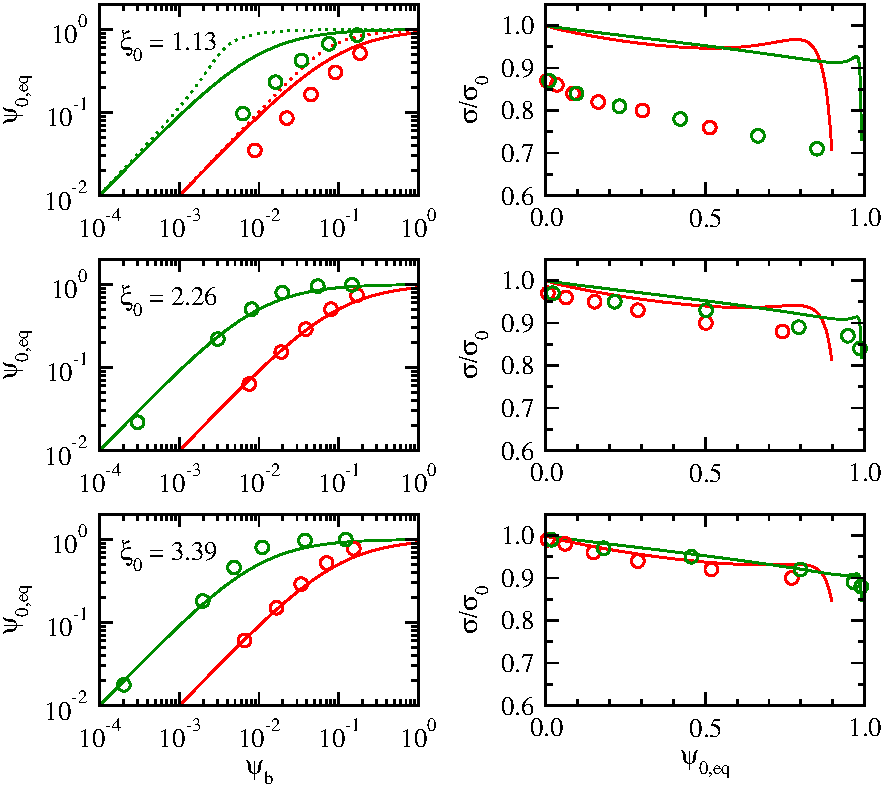
\includegraphics{surfactant_fig1-eps-converted-to.pdf}
\end{center}
\caption{Equilibrium results for one-dimensional simulations with
varying interfacial width $\xi_0$, all other physical parameters
being the same. In particular, $\epsilon = \kappa/4$ and $\beta = 0$.
The
left-hand column shows equilibrium isotherms with $1/K_L$ = 0.1 (red)
and $1/K_L$ = 0.01 (green). The circles are simulations and the lines
the theoretical prediction. The right-hand column shows the
corresponding reduction in surface tension at equilibrium
as a function of $\psi_{0,\mathrm{eq}}$. This reduction is scaled by
the bare interface surface tension $\sigma_0$. The exact result here
is based on a direct numerical integration of the excess free energy
across an equilibrium interfacial profile. The points are computed
by carrying out an analogous numerical integration of the simulated
profile at the given resolution. Note that the representation of
the surfactant porfile is particularly poor at $\xi_0 = 1.13$ as
there turn out to be an even number of lattice points where
$\psi >> \psi_b$ so that the peak value is missed.}
\end{figure}



\subsubsection{Dynamics}

Solve the Ward-Tordai equation.

\subsection{Calibration of the Surface Tension}

The binary fluid model introduces an interfacial tension $\sigma$ which
can be predicted from the choice of free energy \cite{swift,kendon}.
In particular, Kendon et al. 2000 described the process of calibrating
the actual interfacial tension of the model fluid. This was based on
a measurement of the Laplace pressure difference between the fluid
inside and outside a spherical droplet via
\begin{equation}
\Delta p = 2 \sigma / R
\end{equation}
where $R$ is the radius of the spherical drop at equilibrium. This
measurement appears quite difficult in practice owing to tendency of
any initial drop to evaporate \cite{yue2007}.

\subsubsection{New measurement}

Here, we prefer a measure based on the expected profile of the
order parameter $\phi$ and the free energy density at a flat interface.
In order to sample all orientations of the interface with respect to
the lattice we again take a large droplet of fluid A initialised at
rest in fluid B. We assume that the interface is locally flat and so
the procedure holds.

If a droplet with radius $r_0$ is constructed with an initial interfacial
profile of $\phi(r) = \tanh{(r - r_0) / \xi_0}$
with $r$ in the radial direction,  then the free energy density will be
(with $-A = B$)
\begin{equation}
 e(r) = -{\scriptstyle \frac{1}{4}} |A| [1 - \mathrm{sech}^4 (r-r_0)/\xi_0]
+ {\scriptstyle \frac{1}{2}}
 (\kappa/\xi_0^2)\, \mathrm{sech}^4{(r-r_0)/\xi_0}.
\end{equation}
Obtaining a fit to $\xi_0$ from the measured interfacial profile of
$\phi (r)$ and to $ e_0 = \kappa / 2 \xi_0^2$ from the peak in the measured
profile of free energy
density allows an estimate of the interfacial tension to be made:
\begin{equation}
\sigma = 2(8/9)^{1/2} \xi_0 |e_0|.
\end{equation}
This measurement is taken after the initial profile has been allowed
to relax for at least 10 times the larger of the diffusion time
$\xi_0^2 / M$ or the momentum diffusion time $\xi_0^2 / \eta$.


We have measured the surface tension using the following approaches.

\textit{Method 1}.

LB for two distributions with relaxation of order parameter
following Kendon etal. The force on the fluid is applied
via the equilibrium stress following Swift et al.

\textit{Method 2}.

As method 1 but using the realxation of order parameter
following Stratford etal.

\textit{Method 3}.

As Method 1 but with force via divergence of the chemical stress.

\textit{Method 4}.

As Method 3 but with force via divergence of the chemical stress.

\textit{Method 5}.

Using finite difference (1st order upwind) for the order parameter.

\textit{Method 6}.

Using finite difference (3rd order upwind).

\subsubsection{Results}

We follow the parameter sets in Kendon et al Table~2. These
are reproduced here in Table~\ref{tab:r1}. Measured values for
Run028 parameters are show in Table~\ref{tab:newr028}.

\begin{table}
\begin{center}
\begin{tabular}{llllllll}
\hline
Run & $-A, B$ & $\kappa$ & $\eta$ & $M$ & $\sigma$  & $L_0$ & $T_0$ \\
\hline
Rks001 & 0.00625 & 0.004 & 1.41 & 0.05 & 0.0047 & 422 & 1.26e10$^5$\\
Rks002 & 0.00625 & 0.004 & 0.65 & 0.25 & 0.0047 & 89.7 & 1.24e10$^4$\\
Run028 & 0.083 & 0.053 & 1.41 & 0.05  & 0.0625 & 31.8 & 718 \\
Run022 & 0.0625 & 0.04 & 0.5 & 0.25   & 0.0471 & 5.31 & 56.3 \\
Run029 & 0.0625 & 0.04 & 0.2 & 0.15   & 0.0471 & 0.849 & 3.61 \\
Run020 & 0.00625 & 0.004 & 0.025 & 2.00 & 0.00471 & 0.133 & 0.704 \\
Run030 & 0.00625 & 0.004 & 0.0065 & 1.25 & 0.00471 & 0.00829 & 0.0124 \\
Run019 & 0.003125 & 0.002 & 0.0014 & 4.00 & 0.00236 & 0.000831 & 0.000493 \\
Run032 & 0.00125  & 0.0008 & 0.0005 & 5.0 & 0.000943 & 0.000265 & 0.000141\\
\hline  
\end{tabular}
\end{center}
\caption{Table showing common parameter values following Kendon et al.
with the theoretical interfacial tension, $L_0$ and $T_0$. Note that
the order parameter mobility is used here (cf $\tilde{M} = 2M$) in
Kendon et al. (KS values are extra sets used to low 1/$\dot{\gamma}T_0$.)}
\label{tab:r1}
\end{table} 

\begin{table}
\begin{tabular}{lllllll}
\hline
Method & $\xi_0$ & $e_{min}$ & $e_{max}$ & $\sigma$  & $\phi_{min}$
& $\phi_{max}$\\
\hline
\multicolumn{7}{c}{Run028}\\
\hline
Theory   & 1.13 & -0.0207 &  0.0207 & 0.0625 & -1.0 & 1.0 \\
Method 1 & 1.00 & -0.0207 & 0.0128 & 0.063(3) & -1.0091 & 1.0028 \\
Method 2 & 1.00 & -0.0207 & 0.0126 & 0.063(1) & -1.0113 & 0.9993 \\
Method 3 & && & & & \\
Method 4 & && & & & \\
Method 5 & && & & & \\
Method 6 & --& --& --& --& --& --\\
\hline
\multicolumn{7}{c}{Run029}\\
\hline
Theory & 1.13 & -0.0156 & 0.0156 & 0.0471  & -1.0 & 1.0\\
Method 2 & 0.99 & -0.0156 & 0.010(?) & 0.048(4) & -1.0110 & 1.0003\\ 
Method 6 & 1.02 & -0.0156 & 0.0099 & 0.049(0) & -1.0048 & 1.0002\\
\hline
\multicolumn{7}{c}{Run030}\\
\hline
Theory & 1.13 & -0.00156 & 0.00156 & 0.00471 & -1.0 & 1.0\\
Method 2 & 1.04 & -0.00156 & 0.0008(?) & 0.0047(1) & -1.0167 & 1.0063\\
Method 6 & 1.08 & -0.00156 & 0.0007(?) & 0.0048(0) & -1.0028 & 1.0031\\
\hline
\multicolumn{7}{c}{Run019}\\
\hline
Theory & 1.13 & -0.000781 & 0.000781 & 0.00236 & -1.0 & 1.0\\
Method 2 & 1.29(?) & -0.000781 & 0.00015(?) & 0.0022(8) & -1.0312 & 1.0242\\
Method 6 & 1.23(?) & 0.0010(?) &&  0.0024(?) & -1.0085 & 1.0019\\
\hline 
\multicolumn{7}{c}{Run032}\\
\hline
Theory   & 1.13 &  -0.000312 & 0.000312 & 0.000943  & -1.0 &1.0\\
Method 2 & 1.07  & -0.000312& 0.000157 & 0.00094(7) & -1.0511 & 1.0311\\
Method 6 & 1.6(5)& -0.000312 & not st. & 0.0010(7) &-1.0056 & 1.0010\\
\hline
\end{tabular}
\caption{Results for the different methods for Run208 parameters.}
\end{table}

\subsection{User input}

\inputkey{free\_energy surfactant}

Currently under reconstruction.

This is for use with a two order parameter model the first of
which is the composition, as for the symmetric free energy,
while the second $\psi$ represents surfactant concentration.
The free energy density is made up of a number of terms:

\begin{equation}
{\textstyle \frac{1}{2}}A\phi^2
+ {\textstyle \frac{1}{4}}B\phi^4
+ {\textstyle \frac{1}{2}}\kappa (\mathbf{\nabla}\phi)^2
\end{equation}
is the standard symmetric term related to the composition.
These parameters are represented in the input as

\inputkey{surf\_A}
\inputkey{surf\_B}
\inputkey{surf\_kappa}

\begin{equation}
D \left(\psi \ln\psi + (1 - \psi) \ln(1-\psi)\right)
\end{equation}
represents the energy of surfactant in the bulk phase with surfactant
concentration $0 < \psi < 1$ with a single parameter $D$;
\begin{equation}
-{\textstyle \frac{1}{2}} \epsilon \psi (\mathbf{\nabla} \phi)^2
-{\textstyle \frac{1}{2}} \beta \psi^2  (\mathbf{\nabla} \phi)^2
\end{equation}
where the term in $\epsilon$ represents the energy reduction by
adsorbing surfactant at the interface and the term in $\beta$
provides an additional favourable term modelling the fact that
the molecules like to line up; finally, there is an extra term
\begin{equation}
+{\textstyle \frac{1}{2}} W \psi \phi^2
\end{equation}
which is included to stabilise the interface \cite{theissengompper}.

The corresponding keys for the input file are:

\inputkey{D} is the bulk surfactant contribution parameter

\inputkey{epsilon} is the parameter $\epsilon$

\inputkey{W} is the parameter $W$

\inputkey{beta} is the value of the parameter $\beta$.

\inputkey{phi\_b} the initial, uniform, background surfactant
concentration $\psi_b$.

\inputkey{mobility\_psi} Sets the (uniform) mobility for the surfactant
as appropriate for the Cahn-Hilliard equation.



\vfill
\pagebreak
